\begin{question}
    \begin{enumerate}[label=\textbf{\alph*})]
        \item 
        
        \begin{minipage}{\linewidth}
            
            \parbox{.30\linewidth}{
            \centering
            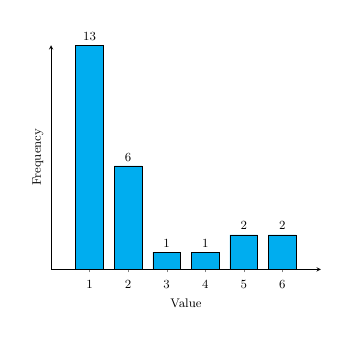
\begin{tikzpicture}[font=\small, scale=0.5]
                \begin{axis}[
                  ybar,
                  bar width=20pt,
                  xlabel={Value},
                  ylabel={Frequency},
                  ymin=0,
                  ytick=\empty,
                  xtick=data,
                  axis x line=bottom,
                  axis y line=left,
                  enlarge x limits=0.2,
                  symbolic x coords={1,2,3,4,5,6},
                  xticklabel style={anchor=base,yshift=-\baselineskip},
                  nodes near coords={\pgfmathprintnumber\pgfplotspointmeta}
                ]
                  \addplot[fill=cyan] coordinates {
                    (1,13)
                    (2,6)
                    (3,1)
                    (4,1)
                    (5,2)
                    (6,2)
                  };
                \end{axis}
            \end{tikzpicture}
            }
            \hfill
            \parbox{.30\linewidth}{
            \centering
            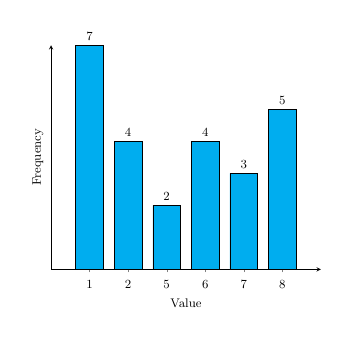
\begin{tikzpicture}[font=\small, scale=0.5]
                \begin{axis}[
                  ybar,
                  bar width=20pt,
                  xlabel={Value},
                  ylabel={Frequency},
                  ymin=0,
                  ytick=\empty,
                  xtick=data,
                  axis x line=bottom,
                  axis y line=left,
                  enlarge x limits=0.2,
                  symbolic x coords={1,2,5,6,7,8},
                  xticklabel style={anchor=base,yshift=-\baselineskip},
                  nodes near coords={\pgfmathprintnumber\pgfplotspointmeta}
                ]
                  \addplot[fill=cyan] coordinates {
                    (1,7)
                    (2,4)
                    (5,2)
                    (6,4)
                    (7,3)
                    (8,5)
                  };
                \end{axis}
            \end{tikzpicture}
            }
            \hfill
            \parbox{.30\linewidth}{
            \centering
            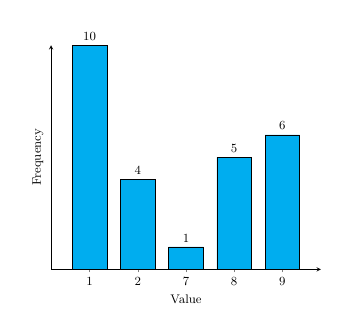
\begin{tikzpicture}[font=\small, scale=0.5]
                \begin{axis}[
                  ybar,
                  bar width=25pt,
                  xlabel={Value},
                  ylabel={Frequency},
                  ymin=0,
                  ytick=\empty,
                  xtick=data,
                  axis x line=bottom,
                  axis y line=left,
                  enlarge x limits=0.2,
                  symbolic x coords={1,2,7,8,9},
                  nodes near coords={\pgfmathprintnumber\pgfplotspointmeta}
                ]
                  \addplot[fill=cyan] coordinates {
                    (1,10)
                    (2,4)
                    (7,1)
                    (8,5)
                    (9,6)
                  };
                \end{axis}
            \end{tikzpicture}
            }
        \end{minipage}

        \item Filtro de suavização pela média
        
        Lembrando: somar todos os elementos e dividir pelo tamanho da 
        kernel (nesse caso por nove)

        \begin{table}[ht]
          \parbox{.45\linewidth}{
            \centering 
            \begin{image}{3}
              1 & 1 & 1 \nl
              1 & 1 & 1 \nl
              1 & 1 & 1 \nl 
            \end{image}
            \caption{Kernel da media}
          }
          \parbox{.45\linewidth}{
            \centering 
            \begin{image}{5}
              * & * & * & * & * \nl
              * & 3 & 4 & 3 & * \nl
              * & 2 & 3 & 3 & * \nl 
              * & 2 & 2 & 2 & * \nl 
              * & * & * & * & * \nl 
            \end{image}
            \caption{Imagem A com suavização pela média}
          }
        \end{table}

        \item Filtro de suavização pela mediana 
      
        Basta encontrar em uma kernel 3x3 o valor de pixel que está no centro 
        da distribuição(mediana)

        \newpage

        \begin{table}[ht]
          \centering 
            \begin{image}{5}
              * & * & * & * & * \nl
              * & 3 & 4 & 2 & * \nl
              * & 1 & 2 & 2 & * \nl 
              * & 1 & 2 & 2 & * \nl 
              * & * & * & * & * \nl 
            \end{image}
            \caption{Imagem A com suavização pela mediana}
        \end{table}

        \item 
        
          $MAX = 255$
          
          $N = 25$

          $r = round(\frac{Somatorio}{n}*MAX)$

          \begin{table}[ht]

            \parbox{.45\linewidth}{
            \centering 
            \begin{tabular}{|c|c|c|c|}
              \hline 
              s & h(s) & Somatório & r \\
              \hline
              1 & 13 & 13 & 133 \\
              \hline
              2 & 6 & 19 & 194 \\ 
              \hline
              3 & 1 & 20 & 204 \\ 
              \hline
              4 & 1 & 21 & 214 \\ 
              \hline
              5 & 2 & 23 & 235 \\ 
              \hline
              6 & 2 & 25 & 255 \\ 
              \hline 
            \end{tabular}
            \caption{Calculando novos valores de A}
            }
            \hfill
            \parbox{.45\linewidth}{
              \centering 
              \begin{image}{5}
                204 & 235 & 194 & 133 & 133 \nl
                133 & 214 & 255 & 194 & 133 \nl
                133 & 133 & 235 & 255 & 194 \nl 
                133 & 133 & 133 & 133 & 133 \nl 
                133 & 194 & 194 & 194 & 133 \nl 
              \end{image}
              \caption{Imagem A com equalização}
            }
          \end{table}

          \begin{table}[ht]

            \parbox{.45\linewidth}{
            \centering 
            \begin{tabular}{|c|c|c|c|}
              \hline 
              s & h(s) & Somatório & r \\
              \hline
              1 & 7 & 7 & 71 \\
              \hline
              2 & 4 & 11 & 112 \\ 
              \hline
              5 & 2 & 13 & 133 \\ 
              \hline
              6 & 4 & 17 & 173 \\ 
              \hline
              7 & 3 & 20 & 204 \\ 
              \hline
              8 & 5 & 25 & 255 \\ 
              \hline 
            \end{tabular}
            \caption{Calculando novos valores de B}
            }
            \hfill
            \parbox{.45\linewidth}{
              \centering 
              \begin{image}{5}
                133 & 71 & 112 & 71 & 255 \nl
                173 & 173 & 133 & 173 & 71 \nl
                112 & 71 & 255 & 204 & 204 \nl 
                173 & 71 & 112 & 255 & 255 \nl 
                204 & 255 & 112 & 71 & 71 \nl 
              \end{image}
              \caption{Imagem B com equalização}
            }
          \end{table}

          \begin{table}[ht]

            \parbox{.45\linewidth}{
            \centering 
            \begin{tabular}{|c|c|c|c|}
              \hline 
              s & h(s) & Somatório & r \\
              \hline
              1 & 10 & 10 & 102 \\
              \hline
              2 & 4 & 14 & 143 \\ 
              \hline
              7 & 1 & 15 & 153 \\ 
              \hline
              8 & 4 & 20 & 194 \\ 
              \hline
              9 & 6 & 25 & 255 \\ 
              \hline
            \end{tabular}
            \caption{Calculando novos valores de C}
            }
            \hfill
            \parbox{.45\linewidth}{
              \centering 
              \begin{image}{5}
                102 & 102 & 255 & 102 & 102 \nl
                102 & 102 & 255 & 194 & 153 \nl
                255 & 255 & 255 & 143 & 102 \nl 
                102 & 102 & 143 & 194 & 194 \nl 
                102 & 143 & 143 & 194 & 255 \nl 
              \end{image}
              \caption{Imagem C com equalização}
            }
          \end{table}

          %%%%%%%%%%%%%%%%%%%% SOBEL %%%%%%%%%%%%%%%%%%%%%%

          \item Sobel 

          \begin{table}[ht]
            \parbox{.45\linewidth}{
              \centering 
              \begin{image}{3}
                -1 & 0 & 1 \nl
                -2 & 0 & 2 \nl
                -1 & 0 & 1 \nl 
              \end{image}
              \caption{Kernel sobel G(x)}
            }
            \parbox{.45\linewidth}{
              \centering 
              \begin{image}{5}
                * & * & * & * & * \nl
                * & -13 & 3 & 14 & * \nl
                * & -13 & -8 & 11 & * \nl 
                * & -5 & -5 & 4 & * \nl 
                * & * & * & * & * \nl 
              \end{image}
              \caption{Imagem A com sobel G(x)}
            }
          \end{table}

          \newpage

          \begin{table}[ht]
            \parbox{.45\linewidth}{
              \centering 
              \begin{image}{3}
                -1 & -2 & -1 \nl
                0 & 0 & 0 \nl
                1 & 2 & 1 \nl 
              \end{image}
              \caption{Kernel sobel G(y)}
            }
            \parbox{.45\linewidth}{
              \centering 
              \begin{image}{5}
                * & * & * & * & * \nl
                * & 7 & -7 &  -14 & * \nl
                * & -11 & 14 & 7 & * \nl 
                * & 1 & 9 & 12 & * \nl 
                * & * & * & * & * \nl 
              \end{image}
              \caption{Imagem A com sobel na direção Y}
            }
          \end{table}

          \begin{table}[ht]
            \centering 
            \begin{image}{5}
              * & * & * & * & * \nl
              * & 20 & 10 &  28 & * \nl
              * & 24 & 22 & 18 & * \nl 
              * & 6 & 14 & 16 & * \nl 
              * & * & * & * & * \nl 
            \end{image}
            \caption{Imagem A com sobel $|G(x)| + |G(y)|$}
          \end{table}

        \end{enumerate}
\end{question}